\documentclass[17pt]{extarticle}

\usepackage{extsizes}

\usepackage[paperheight=9.6cm,paperwidth=17cm,margin=0.8cm]{geometry}
\parindent=0mm \parskip=3.2mm \linespread{1.15}

\usepackage{amsmath,amssymb,mathtools}
\usepackage{graphicx,xcolor,tikz}
\usetikzlibrary{positioning}
\usepackage[linguistics]{forest}
\usepackage{enumerate,enumitem}

\setlist{leftmargin=*}
\usepackage[russian]{babel}

\definecolor{fon}{HTML}{0f1622} % {2f3642}
\definecolor{bluetri}{RGB}{45,155,190}

\pagecolor{fon}
\color{white}

\usepackage{mathspec}

\setmainfont[
	Path = f/,
	BoldFont=ib.ttf,
	ItalicFont=ii.ttf,
	BoldItalicFont=ibi.ttf
		]{i.ttf}
		
\setmathfont(Digits)[Path = f/]{i.ttf}
\setmathfont(Latin)[Path = f/]{ii.ttf}
\setmathfont(Greek)[Path = f/, Uppercase]{g.ttf}
\setmathfont(Greek)[Path = f/, Lowercase]{g.ttf}



\DeclarePairedDelimiter\lr{(}{)}
\newcommand{\newslide}[1]{\newpage \begin{center} \large #1 \end{center}}
\newcommand{\tr}[1]{\textcolor{red}{#1}}

\DeclareMathOperator{\rlbl}{relabel}
\DeclareMathOperator{\size}{size}
\DeclareMathOperator{\length}{length}
\DeclareMathOperator{\Rel}{Rel}
\DeclareMathOperator{\Rlbl}{Relabel}
\DeclareMathOperator{\Inse}{Insert}

\begin{document}

\ \\ [1cm]

\begin{center} {\Large Dynamic Voronoi Diagrams} \bigskip \\
	{\large B. Zolotov, Young Researchers Seminar} \end{center}

\newslide{Voronoi Diagrams} \vspace{-6mm}

\begin{center}
	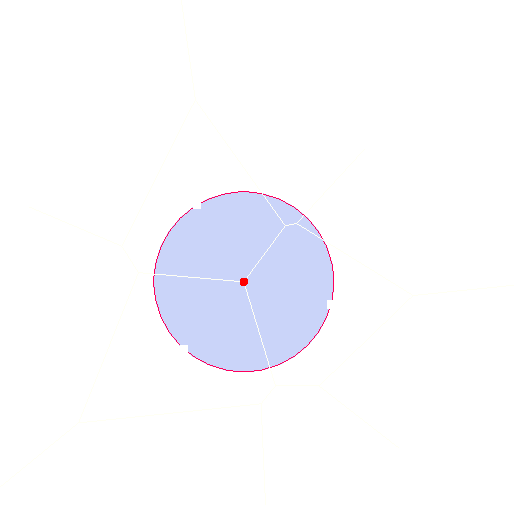
\includegraphics[height=5.3cm]{figs/voronoiCircle-dark}
\end{center}

\newslide{Voronoi Diagrams}

\begin{itemize}
	\item Every point belongs to the region of the closest {\it site},
	\item Have clear applications everywhere,
	\item Can be generalized for other metrics.
\end{itemize}

\newslide{Explicit Dynamic Voronoi Diagrams}

There can be \(Ω (n)\) changes in coordinates \\
per addition of a site, so time \\
better than \(O (n)\) is impossible.

\newslide{Implicit Dynamic Voronoi Diagrams}

($=$ Nearest neighbor query)

\begin{itemize}
	\item Kaplan, Mulzer, Roditty, Seiferth, Sharir 2020
	\item Chan, 2010
\end{itemize}

\newslide{Combinatorial Dynamic Voronoi Diagrams}

Maintain the graph of the Voronoi diagram.

Maybe there is a sublinear algorithm for \\
inserting a site; the coordinates of all \\
the vertices can be output in \(O(n)\).

\newslide{Flarb} \vspace{-6mm}

When inserting a new site into a Voronoi diagram, \\
you basically throw out everything inside \\
new site's cell and replace it with a cycle. \\
This is called a flarb.

The point is, you do not need to change \\
every cell to implement a flarb.

\newslide{Combinatorial changes} \vspace{-7mm}

Only those cells need combinatorial changes \\
whose Voronoi circles enclose the new site.

\begin{center}
	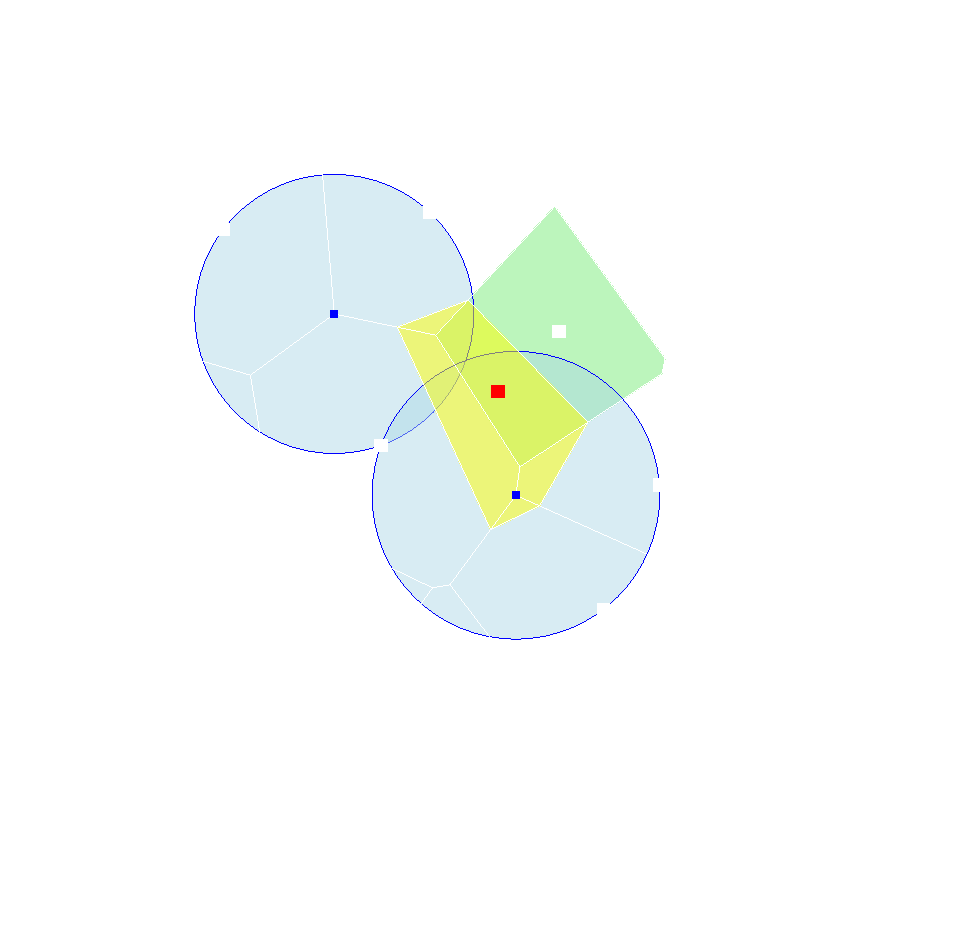
\includegraphics[height=4.7cm]{figs/identChanges-dark}
\end{center}

\newslide{Chan's polylog structure} \vspace{-5mm}

Given a set of points in \( \mathbb R^3 \), find extreme of them in given direction: polylog time for addition and queries.

\begin{itemize}
	\item Smallest enclosing circle
	\item Width of a set; convex layers
	\item {\it Report a circle containing \(q\)}
\end{itemize}

\newslide{Potential function}
\[ Φ = λ \cdot \sum\limits_{i=1}^n
   \min\left\{
      \size(f_i), \sqrt{n}
   \right\}\]

When a flarb is applied, all cells that \\
undergo combinatorial changes reduce in size.

\newslide{\(\sqrt{n}\) lower bound}

\begin{center}
	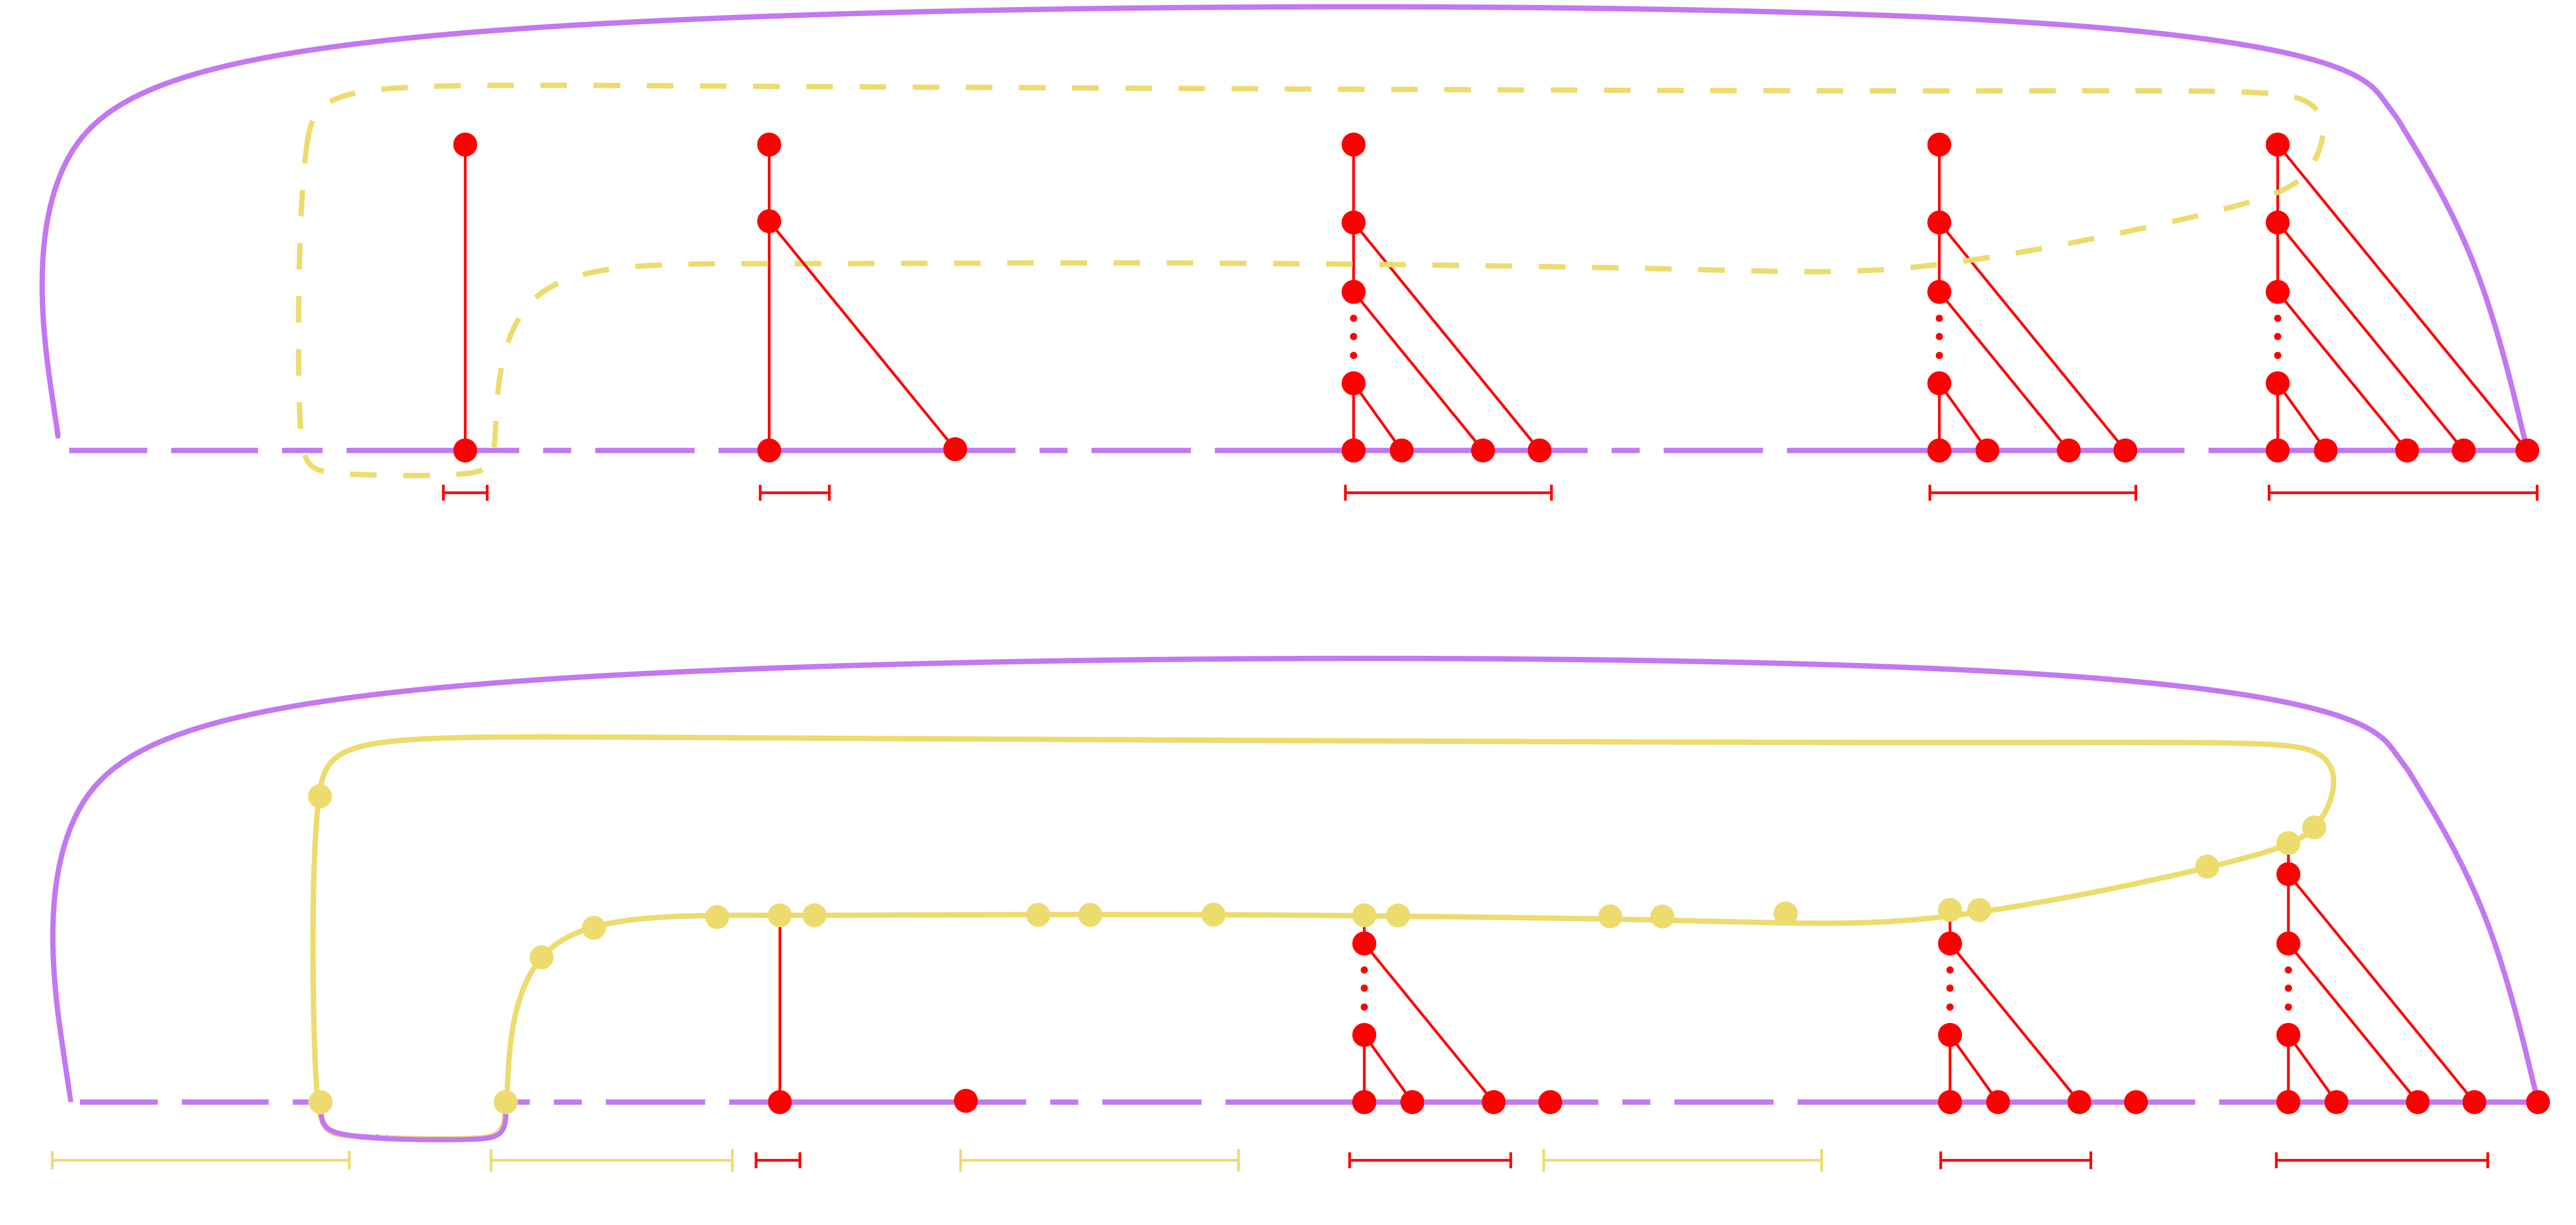
\includegraphics[width=0.85\textwidth]{figs/sqrtn}
\end{center}

\newslide{VD for several points and a line}

\begin{center}
	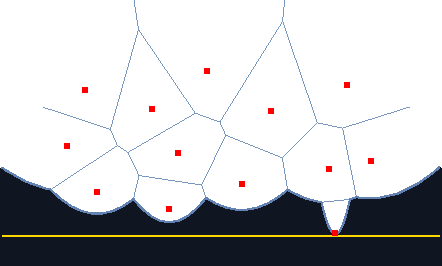
\includegraphics[width=0.65\textwidth]{figs/bl-ex-dark}
\end{center}

\newslide{Relabel operation}

\begin{center}
	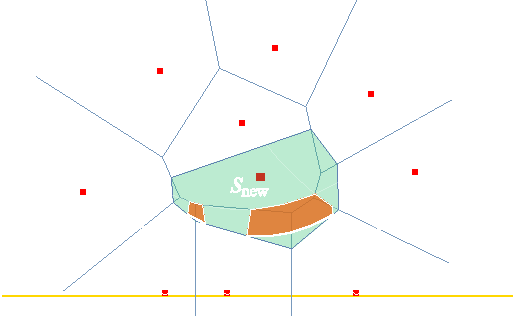
\includegraphics[width=0.65\textwidth]{figs/combchange-dark}
\end{center}

\newslide{Beach line and D—S sequences} \vspace{-7mm}

This configuration of parabolas corresponds \\
to the sequence \( fabacdafghgkgf \).

\begin{center}
	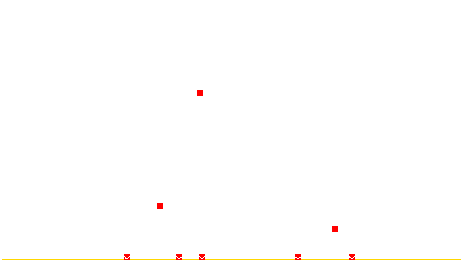
\includegraphics[height=4.6cm]{figs/parab-config-dark}
\end{center}

\newslide{D—S sequences and trees} \vspace{-7mm}
\[ fabacdafghgkgf \] \vspace{-16mm}

\begin{center}
	\begin{forest} for tree={circle, draw, white, minimum size=0.8ex, inner sep=0.08ex,% 
	   l=1.55cm, s sep=1.6mm}
		[$f$ [$a$ [$b$] [$c$] [$d$]] [$g$ [$h$] [$k$]]]
	\end{forest}
\end{center}


\newslide{The order of relabels}

\begin{center}
	\begin{forest} for tree={circle,draw,white,minimum size=0.7ex,%
		inner sep=0.4ex,l=1.5cm,s sep=2.7mm}
	   [ ,alias=ROOT
	      [ ,fill=bluetri!65!gray,alias=RA
	         [ ,before drawing tree={x-=0.7cm}]
	         [ ,before drawing tree={x-=0.7cm}]
	         [ ,before drawing tree={x-=0.35cm},alias=A
	            [ ,fill=bluetri!65!gray,alias=RB] [ ] [ ]]
	      ] [ [ ]]
	      [
	         [ [ ]]   [ ]   [ [ ] [ ]]   [ ]
	      ]
	   ]
	  	\node[left=-0.05cm of A]{$a$};
		\node[right=-0.05cm of A]{$a$};
		\node[left=-0.05cm of RA]{$s_j$};
		\node[left=-0.05cm of RB]{$s_j$};
	\end{forest}
\qquad
	\begin{forest} for tree={circle,draw,white,minimum size=0.7ex,%
		inner sep=0.4ex,l=1.5cm,s sep=2.7mm}
	   [ ,alias=ROOT
	      [
	         [ ,before drawing tree={x-=0.45cm}]
	         [ ,before drawing tree={x-=0.45cm}]
	         [ ,fill=bluetri!65!gray,alias=RA
	            [ ,fill=bluetri!65!gray]
	            [ ,fill=bluetri!65!gray]
	            [ ]]
	      ] [ [ ]]
	      [ ,alias=A
	         [ [ ]]
	         [ ]
	         [ ,fill=bluetri!65!gray,alias=RB
	            [ ,fill=bluetri!65!gray] [ ,fill=bluetri!65!gray]]
	         [ ,before drawing tree={x+=0.45cm}]
	      ]
	   ]
		\node[left=-0.05cm of RA]{$s_j$};
		\node[right=-0.05cm of RB]{$s_j$};
		\node[left=-0.05cm of A]{$a$};
		\node[right=-0.05cm of A]{$a$};
	\end{forest}
\end{center}


\newslide{Possible set of relabels} \vspace{-15mm}

\begin{center}
	\begin{forest} for tree={circle,draw,white,minimum size=0.7ex,%
		inner sep=0.4ex,l=1.2cm,s sep=3.6mm}
	   [
	      [ ,fill=bluetri!65!white
	         [ ]
	         [ ,fill=bluetri!65!white]
	         [ ,fill=bluetri!65!white
	            [ ] [ ,fill=bluetri!65!white] [ ]]
	      ] [ [ ]]
	      [ ,fill=bluetri!65!white
	         [ [ ]]   [ ,fill=bluetri!65!white]
	         [ ,fill=bluetri!65!white [ ,fill=bluetri!65!white] [ ,fill=bluetri!65!white]]
	         [ ]
	      ]
	   ]
	\end{forest}
\end{center}
 \vspace{-2mm}

Nodes that are relabelled form a union of subtrees, \\
whose roots are children of a single node \(R\).

\newslide{Inserts and sizes of nodes / the length} \vspace{-6mm}

	An {\it insert} is a relabel that does not reduce the size of the node it is applied to. \vspace{-3mm}

\begin{itemize}
	\item When an insert is applied to a sequence, \\
	   the length of the sequence increases by 1.
	\item When a relabel that is not an insert is applied \\
	   to a sequence, the length of the sequence \\
	   may decrease, but by at most 2.
\end{itemize}

\newslide{Potential function}
   \[
	Φ = 3 \cdot \sum\limits_{i=1}^n
	\min\left\{ \size(s_i), 2 \sqrt{n} \right\}
	- \length (S).
   \]

This accounts for the changes in the sizes of nodes \\
and in the length of the sequence.

\newslide{Further research}

It suspiciously seems like you can only \\
have significantly less than $\sqrt{n}$ \\
relabels per letter…

\end{document}
